\section{DEEP RL WITH WORLD MODELS}\label{approach}

In this section, we reintroduce the World Models architecture \cite{ha2018recurrent} in the context of reinforcement learning. A trained World Model can be incorporated in the RL training loop as shown in \cref{fig:worldmodel} to transform an image observation into a compressed representation that is then passed to the agent. This output consists of a latent encoding $z_t$ of the image from a VAE and the hidden state $h_t$ from a Gaussian Mixture Density RNN (MDRNN). The concatenation of these two vectors becomes the state feature representation, which the agent can treat as the environment's underlying state when learning an optimal policy.
\begin{figure}[h]
	\centering
	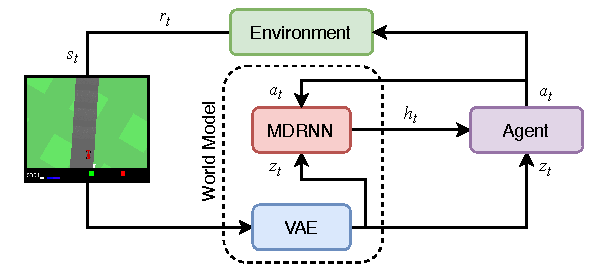
\includegraphics[width=0.49\textwidth]{images/worldmodel2.pdf}
	\caption{MDP Loop with a World Model}\label{fig:worldmodel}
\end{figure}

\subsection{VAE Model}

A VAE consists of an encoder network that compresses an input image $s_t$ into a latent feature vector $z_t$, and also a decoder network to reconstructed the image from the preserved features as shown in \cref{fig:vae}. The VAE parameterized by $\theta$ is trained to minimize the difference between the reconstructed image and the input image with the constraint of minimizing the KL divergence between the latent encoding space and the normal distribution which was found to suitable prior over the latent variable $z$ for maximum-likelihood feature representation~\cite{diederik2014auto}. This is achieved by minimizing the following loss function: 
\begin{equation}
    L_{\mathrm{VAE}}(s_t;\theta) = (s_t - \hat{s_t})^2 + D_{\mathrm{KL}}(p(z_t \mid s_t)\,\|\,\mathcal{N}(0,1)),
\end{equation}
where the first term minimizes the difference between the reconstructed and input image and the second term penalizes large shifts in the conditional latent state distribution $p(z_t \mid s_t)$ from a unit normal. A VAE is ideal for this task as it learns to encode the most important sources of variation from the distribution of training images within a small linear vector. The KL divergence term ensures that the model is able to sufficiently represent less frequent states without overfitting to a particular region of the state space.
\begin{figure}[h]
	\centering
	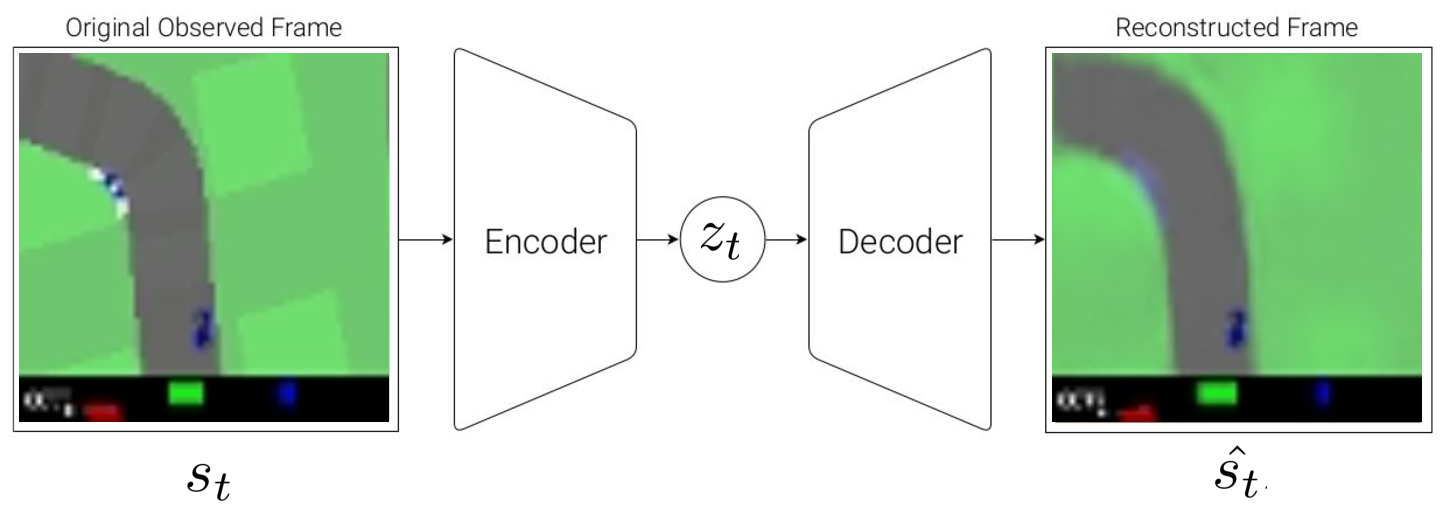
\includegraphics[width=0.49\textwidth]{images/vaes.pdf}
	\caption{Flow diagram of a VAE \cite{ha2018recurrent}}\label{fig:vae}
\end{figure}

\subsection{MDRNN Model}

While the VAE transforms a high-dimensional image into a low dimensional latent vector, it is only a static representation at a single point in time and lacks information about the temporal dynamics of the environment. Therefore, an RNN is trained to encode temporal information over a sequence of latent vectors. \Citeauthor{ha2018recurrent} utilized a Long-Short-Term-Memory (LSTM) to model the temporal changes in the next state through its hidden LSTM state $h_{t+1}$ calculated from the current latent vector $z_t$, chosen action $a_t$ and its current hidden state $h_t$~\cite{ha2018recurrent}. As the distribution of next states is often stochastic, the output of the LSTM is passed to a Gaussian-Mixture Density Network (MDN) \cite{bishop1994mixture} represented in \cref{fig:mdrnn} as a linear layer which outputs the mean $(\mu)$, standard deviation $(\sigma)$, and mixing weights $(\textbf{w})$, for a specified number of Gaussian distributions. The predicted next latent state can be sampled by first sampling a Gaussian index from the mixture weights $w$ and then sampling the latent vector $\hat{z}_{t+1}$ from the selected Gaussian. 
\begin{figure}[h]
	\centering
	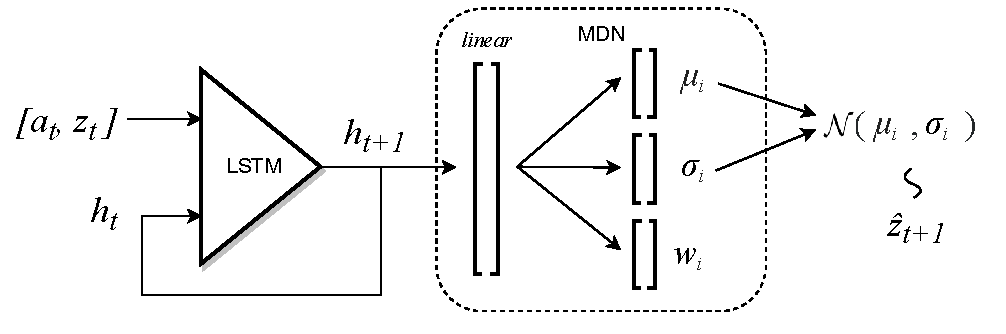
\includegraphics[width=0.5\textwidth]{images/MDRNN2.pdf}
	\caption{Flow diagram of a MDRNN}\label{fig:mdrnn}
\end{figure}

The MDRNN can be modeled as a function parameterized by $\beta$ defined as $ M(a_t,z_t;h_t;\beta) \rightarrow h_{t+1}, \hat{z}_{t+1},$ where $z$ is sampled from $\mathcal{N}(\mu_i, \sigma_i)$, and $i$ is sampled from a categorical distribution with probabilities \textbf{w} \cite{ellefsen2019mixture}. Given an experience tuple $(s_t, a_t, s_{t+1}, r_t, d_t)$, the latent states $z_t$ and $z_{t+1}$ can be obtained as the output of a trained VAE given inputs $s_t$ and $s_{t+1}$. Then, with the probability $p(z_{t+1} \mid \mu,\sigma;\beta)$ of sampling $z_{t+1}$ from $\mu$ and $\sigma$, the MDRNN $M$ can be trained by minimizing the following loss function:
\begin{dmath}
	L_{\mathrm{MDRNN}}(\beta) = -\mathbb{E}_{(z,z') \sim \mathrm{VAE}(\mathcal{E}),\ a \sim \mathcal{A},\ (\mu,\sigma,w) \sim M(a,z)} \\ \left[ \log \left( \sum^n_i w_i \ p(z' | \mu_i,\sigma_i;\beta) \right) \right] 
\end{dmath} 

\subsection{Controller Model}\label{sec:ctrl}

The controller model is a simple linear mapping of the latent state from the World Model to an action. It was noted in \cite{ha2018recurrent} that the hidden state of the MDRNN $h_t$ was sufficient for encoding temporal information of the current state since it is used to predict $\hat{z}_{t+1}$ from $z_t$ and $a_t$. As a result, the controller can be represented as a linear function $a_t = W_c \cdot [z_t, h_t] + b_c$ where $W_c$ is the weight and $b_c$ is the bias for the single-layer network. As the controller is designed to have the minimum number of parameters for a linear function of $[z_t, h_t]$, it can be optimized with the CMA-ES algorithm. In this paper, the controller is not considered part of the World Model, but instead as a baseline agent for benchmarking deep RL agents trained with the World Model.

\subsection{Training The World Model}

Since the variation in the image observation space is stationary over time for a fixed policy, this allows the VAE to be trained independently from the MDRNN. Similarly, as the controller is responsible only for policy optimization, it can be trained with simplified states from a pre-trained World Model. \cref{alg:wm} outlines the procedure for training each component of the World Model. Upon initializing the parameters of the VAE $V$, MDRNN $M$, and Controller $C$ with the appropriate \textsc{InitParameters} function, a dataset $\mathcal{D}$ is extended with $N$ trajectories sampled from the environment $\mathcal{E}$ using $C$ as the policy. Then, with learning rate $\alpha$, $V$ is trained on batches of images from $\mathcal{D}$. $M$ can then be trained using the previously trained $V$ to compress images to latent vectors. $C$ is then optimized using \textsc{CMA-ES} given a trained World Model ($V$,$M$). It is possible that one iteration of this training process is not enough to encounter optimal states of the environment since the initial trajectories are sampled with a random controller. Hence, this loop is repeated using the previously trained controller and World Model for a specified $S$ iterations depending on the complexity of the environment.

\section{DEEP RL WITH WORLD MODELS}

This section describes the process of training RL agents using a trained World Model, as well as the architecture of the RL algorithms to be trained with the World Model.

\subsection{Training RL Agents With The World Model}

Given a pre-trained World Model as the output from \cref{alg:wm}, the RL agent can focus solely on identifying the optimal mapping from latent features to actions that maximize total reward. \cref{alg:rl} describes the procedure for stepping through the environment $\mathcal{E}$ with a World Model consisting of the VAE $V$ and MDRNN $M$ that are either trained using \cref{alg:wm} or loaded from a previously trained World Model on the same environment $\mathcal{E}$. Then, the training of an RL policy $\pi$ towards an optimal policy occurs over a specified number of training trajectories. At the start of each training trajectory, the MDRNN hidden state $h$ is initialized with \textsc{InitHidden}, the initial observation $s$ is sampled from the environment with \textsc{InitState}, and the latent encoding $z$ of the initial image observation is sampled from the VAE. The flag $d$ signifying reaching a terminal state is initialized to false. Then, until a terminal state is reached, the RL training loop proceeds with the \textsc{Step} function applying each agent action $a$ to the environment and outputting the next observation $s'$, reward $r$ and updated terminal flag $d$. The observations $s$ and $s'$ are replaced with the latent state $[z,h]$ and next latent state $[z',h']$, where $z$ and $h$ are the outputs of the VAE $V$ and MDRNN $M$ respectively. The agent is then given the updated experience tuple with latent states using the where it can store or use in a training update through the \textsc{Train} function implemented according to a specified RL algorithm.

\begin{algorithm}[t]
   % \SetAlgoLined
    \caption{Training Loop for World Model}\label{alg:wm}
    \begin{algorithmic}[1] 
        \Procedure{TrainWorldModel}{$\mathcal{E}, S, N$} 
            \State $ V(s;\theta) \gets \Call{InitParameters}{\theta} $
            \State $ M(z,a;\beta) \gets \Call{InitParameters}{\beta} $
		    \State $ C(z,h;W_c, b_c) \gets \Call{InitParameters}{W_c, b_c} $
		    \State $ \mathcal{D} \gets \emptyset $
            \For{$ i \textbf{ in } \{1, \ldots, S\}$} 
                \State $\mathcal{D} \gets \mathcal{D} \cup \Call{SampleTrajectories}{\mathcal{E},C,N}$
                \For{$ batch $ $\textbf{in}$ $\mathcal{D}$}
    				\State $ \mathcal{L}_{\theta} \gets L_{\mathrm{VAE}}(batch;\theta) $
    				\State $ \theta \gets \theta - \alpha \nabla \mathcal{L}_{\theta}$
			    \EndFor
                \For{$ batch $ $\textbf{in}$ $\mathcal{D}$}
    				\State $ \mathcal{L}_{\beta} \gets L_{\mathrm{MDRNN}}(V,batch;\beta) $
				    \State $ \beta \gets \beta - \alpha \nabla \mathcal{L}_{\beta}$
			    \EndFor
			    \State $ C \gets \Call{CMA_ES}{C,V,M} $
            \EndFor
            \State \textbf{return} $V, M$
        \EndProcedure
    \end{algorithmic}
\end{algorithm}

\begin{algorithm}[t]
    %\SetAlgoLined
    \caption{RL Training With Trained World Model}\label{alg:rl}
    \begin{algorithmic}[1] 
        \Procedure{TrainRLAgent}{$\mathcal{E}, S, N$} 
            \State $ V, M \gets \Call{TrainWorldModel}{\mathcal{E}, S, N} $
            \State $ \pi(z,h;$\textbf{$\phi$}$) \gets \Call{InitParameters}{\phi} $
            \For{$ \textrm{each trajectory} $ $\textbf{do}$} 
                \State $ h \gets \Call{InitHidden}{M} $
    			\State $ s \gets \Call{InitState}{\mathcal{E}} $
    			\State $ z \gets V(s;\theta) $
    			\State $ d \gets $ false
    			\While{$ d =$ false}
    			    \State $ a \gets \pi([z,h];\phi) $
    				\State $ s', r, d \gets \Call{Step}{\mathcal{E}, a}$
    				\State $ h' \gets M(z,a;h;\beta) $
    				\State $ z' \gets V(s';\theta) $
    				\State $ \Call{Train}{\pi, ([z,h], a, [z',h'], r, d)} $
    				\State $ [z,h] \gets [z',h'] $
    			\EndWhile
            \EndFor
        \EndProcedure
    \end{algorithmic}
\end{algorithm}

\begin{figure*}[ht!]
	\centering
    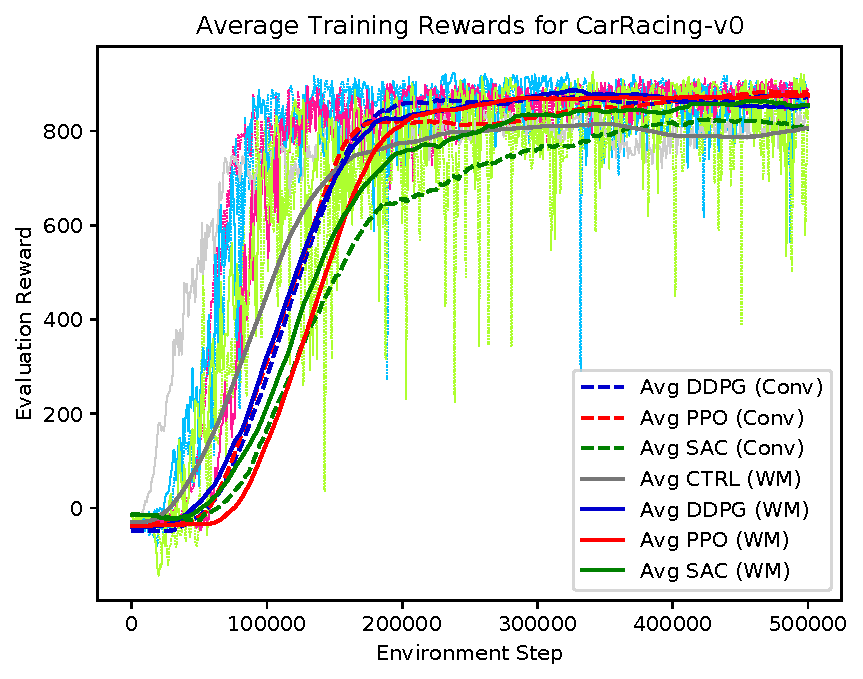
\includegraphics[width=0.325\linewidth]{images/CarRacing-v0.pdf}
    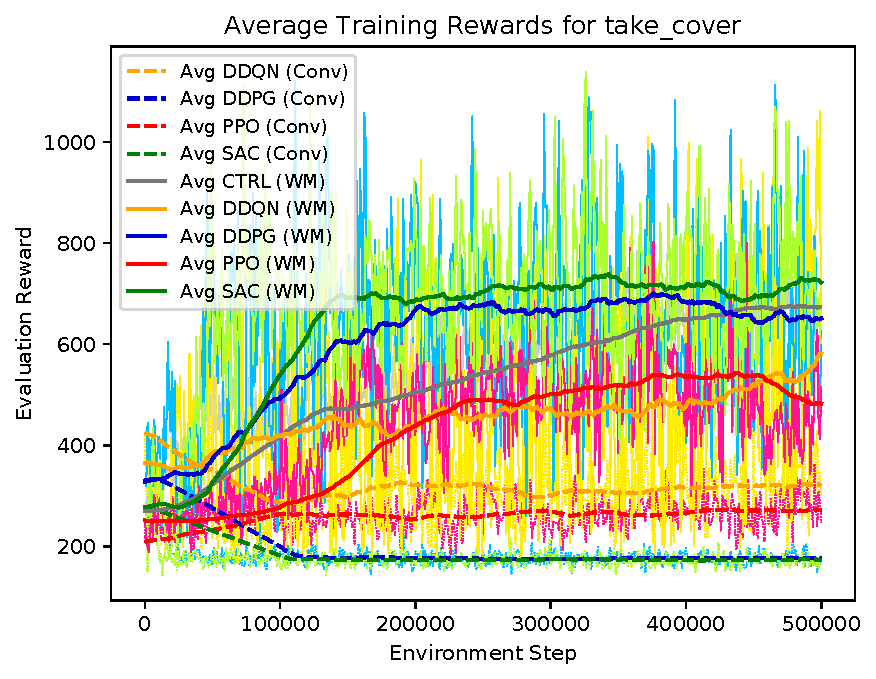
\includegraphics[width=0.33\linewidth]{images/take_cover.pdf}
    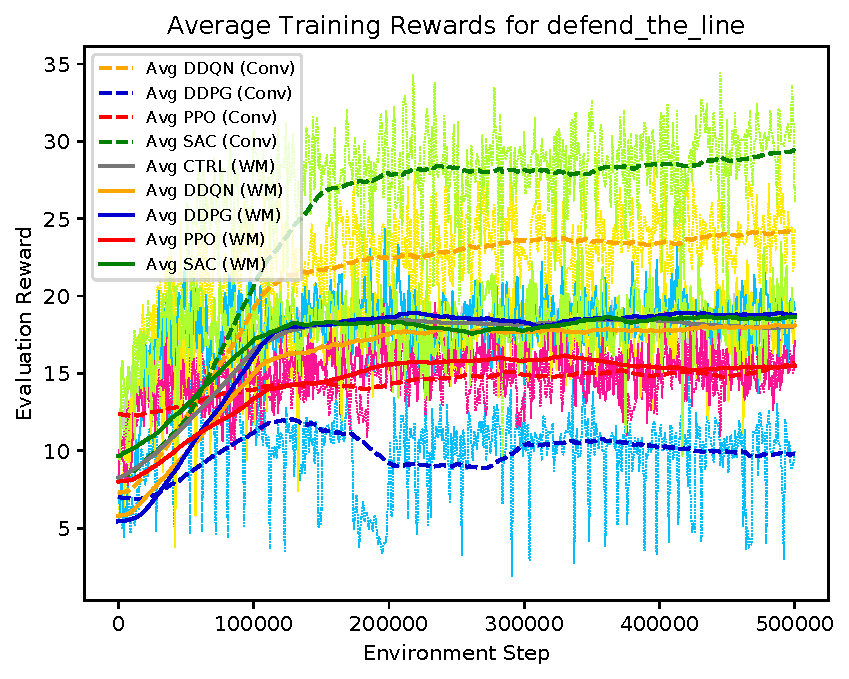
\includegraphics[width=0.32\linewidth]{images/defend_the_line.pdf}
    \caption{The rolling average evaluation rewards over the previous $100000$ steps for different RL algorithms trained in the CarRacing-v0 (left), take_cover (mid), and defend_the_line (right) environments. In each plot, the solid thick lines represent training with the pre-trained World Model and dashed thick lines represent training using convolutional layers. The thin lines represent evaluation rewards every $1000$ steps.}\label{fig:res}
\end{figure*}

\subsection{RL Agent Architecture}

The RL algorithms to be trained with the World Model include Double DQN (DDQN)~\cite{wang2015dueling}, DDPG~\cite{lillicrap2015continuous}, PPO~\cite{schulman2017proximal}, and SAC~\cite{haarnoja2018soft}. These agents will be tested first with raw grey-scale image inputs to evaluate the baseline performance of learning an environment representation along with the learning of the optimal policy. For the baseline, each state input will consist of the current image observation stacked on top of the two previous observations. Then, the architecture of the baseline actor and critic will consist of a convolutional component to reduce the 2D image to a 1D vector which is then passed to a feed-forward component which will output the desired action or state-value. The convolutional component will share the same network architecture as the VAE encoder having four convolutional layers. The feed-forward component will consist of three layers to map the output of the convolutional component or world model to the desired output size of the actor or critic.

All agents will be trained on batches of experience tuples from $16$ parallel environments as done in~\cite{mnih2016asynchronous}. An experience replay buffer of a maximum size $100000$ samples will be used for off-policy algorithms DDQN, DDPG and SAC. DDQN and DDPG rely on explicit random exploration schedules which will be implemented with a Brownian noise process where the scale of noise is reduced from $1.0$ to a minimum of $0.02$ at a decay rate of $0.98$ after each trajectory.\footnote{The complete implementation is available on Github at https://github.com/sisl/WorldModelsForDeepRL} %https://github.com/shawnmanuel000/WorldModelsForDeepRL}